\documentclass[conference]{IEEEtran}
\IEEEoverridecommandlockouts
% The preceding line is only needed to identify funding in the first footnote. If that is unneeded, please comment it out.
\usepackage{cite}
\usepackage{amsmath,amssymb,amsfonts}
\usepackage{algorithmic}
\usepackage[spanish]{babel}
\usepackage[utf8]{inputenc}
\usepackage{graphicx}
\usepackage{textcomp}
\usepackage{xcolor}
\def\BibTeX{{\rm B\kern-.05em{\sc i\kern-.025em b}\kern-.08em
    T\kern-.1667em\lower.7ex\hbox{E}\kern-.125emX}}
\begin{document}

\title{
{\large \textsc{Escuela Superior Politécnica del Litoral}\\
Administración de Sistemas Operativos - CCPG1031: Proyecto Final 
}\\
Implementación de Servicio de
Telefonía IP (VoIP)\\
}

\author{\IEEEauthorblockN{\textbf{Lino Ontano}}
\IEEEauthorblockA{	\textit{Telemática}
\\Guayaquil - Ecuador \\
lontano@espol.edu.ec
}
\and
\IEEEauthorblockN{\textbf{Flavio Murillo}}
\IEEEauthorblockA{	\textit{Telemática}
\\Guayaquil - Ecuador \\
famurill@espol.edu.ec
}
\and
\IEEEauthorblockN{\textbf{Jonathan Yagual}}
\IEEEauthorblockA{	\textit{Telemática}
\\Guayaquil - Ecuador \\
jonosyag@espol.edu.ec
}
}


\maketitle
\begin{abstract}
	Este proyecto permitirá aprender las bases necesarias para la elaboración de una central telefónica (PBX) con software gratuito.
\end{abstract}

\begin{IEEEkeywords}
	PBX
\end{IEEEkeywords}
\section{Introducción}\label{sec:int}
Se ha oído hablar mucho de VoIP, con aplicaciones tan extendidas como Skype. Sin embargo,
la propuesta en este proyecto es ir algo más allá y poner en funcionamiento nuestra propia
centralita telefónica PBX basada en VoIP. Montar una centralita telefónica propia implica
un ahorro de dinero en la compra de una centralita convencional o de VoIP, para ello se utlizará Asterisk, software distribuido bajo licencia GNU. Entre
las funcionalidades de Asterisk, es posible montar, incluso, sistemas de atención automática,contestador e integrar la telefonía IP en nuestra sitio web.
En el presente proyecto instalaremos un servidor PBX Asterisk paso a paso, configuración de su GUI FreePBX y conectaremos clientes SoftPhones para simular la funcionalidad de nuestra central telefónica.


\section{Antecedentes}\label{sec:ant}
\subsection{\textbf{ VoIP:}} 
\textbf{Voz sobre protocolo de Internet} es un conjunto de recursos que hacen posible que la señal de voz viaje a través de Internet empleando el protocolo IP, es decir la señal se envía en forma digital, en paquetes de datos. Los protocolos de internet que se usan para enviar las señales de voz sobre la red IP se conocen como protocolos de voz sobre IP o protocolos IP. 
Es muy importante diferenciar entre voz sobre IP (VoIP) y telefonía sobre IP.
\begin{itemize}
\item VoIP es el conjunto de normas, dispositivos, protocolos ―en definitiva, la tecnología― que permite transmitir voz sobre el protocolo IP.
\item La telefonía sobre IP es el servicio telefónico disponible al público, por tanto con numeración E.164, realizado con tecnología de VoIP.\footnote{Tampoco se debe confundir «telefonía sobre IP» con ToIP (text over IP: ‘texto sobre IP’).}
\end{itemize}
\begin{figure}[h]
	\centerline{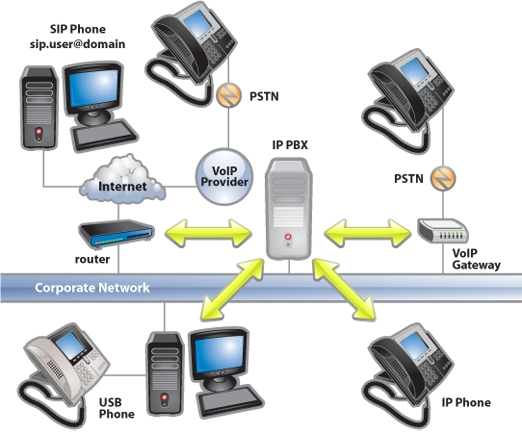
\includegraphics[width=0.3\textwidth]{img/voip01.jpg}}
	\caption{Componentes de una central telefónica VoIP}
	\label{fig:ant01}
\end{figure}
Los elementos que forman parte de un servicio VoIP son los siguientes:
\begin{itemize}
\item \textbf{Cliente}: es el que establece las llamadas de voz, se recibe a través del micrófono del usuario (entrada de información) se codifica, se empaqueta y, de la misma forma, esta información se decodifica y reproduce (salida de la información).\\
Un cliente puede ser un usuario de Skype o un usuario de alguna empresa que venda sus servicios de telefonía sobre IP o teléfonos IP o \textit{Softphones} que es un software que permite realizar llamadas a través de una computadora conectada a internet.

\item \textbf{Servidores}: son los que se encargan de manejar operaciones de base de datos, realizado en un tiempo real como en uno fuera de él. Entre estas operaciones se tienen la contabilidad, la recolección, el enrutamiento, la administración y control del servicio, el registro de los usuarios.\\
Usualmente en los servidores se instala software denominados Switches o IP-PBX (conmutadores IP), ejemplos de switches pueden ser "Voipswitch", "Mera", "Nextone" entre otros, y de IP-PBX pueden ser los de Alcatel-Lucent, Cisco o Avaya en marcas comerciales y Asterisk de código abierto. Para el presente proyecto se utilizará Asterisk.
\item \textbf{Gateways}: brindan un puente de comunicación entre todos los usuarios, su función principal es la de proveer interfaces con la telefonía tradicional adecuada, la cual funcionará como una plataforma para los usuarios (clientes) virtuales. Los gateways se utilizan para terminar la llamada, es decir: el cliente origina la llamada y el gateway termina la llamada, eso es cuando un cliente llama a un teléfono fijo o celular, debe existir la parte que hace posible que esa llamada que viene por internet logre conectarse con un cliente de una empresa telefónica fija o celular.
\end{itemize}
\subsection{\textbf{ IP-PBX:}}  
Un conmutador IP o PBX por sus siglas en inglés de “Private Branch eXchange”, es la evolución de los viejos conmutadores basados en TDM; una red telefónica privada que es utilizada dentro de una empresa. En la actualidad, la era de las Comunicaciones Unificadas, los conmutadores IP ya no son simples plataformas de voz como lo eran antes. Un línea muy delgada separa las Comunicaciones Unificadas y la Telefonía IP.\\
Un Conmutador IP o PBX IP conecta las extensiones internas dentro de una empresa y al mismo tiempo las conecta con la red pública conmutada, conocida también como PSTN (Public Switched Telephone Network), Proveedores VoIP y Troncales SIP, como se observa en la figura \ref{fig:ant01}.
\subsection{\textbf{ Asterisk:}}
\begin{figure}[h]
	\centerline{
\includegraphics[width=0.2\textwidth]{img/asterisk01.png}}
	\caption{Logo de Asterisk}
	\label{fig:ant02}
\end{figure}
\textit{Asterisk} es un programa de software libre (bajo licencia GPL) que proporciona funcionalidades de una central telefónica (PBX). Como cualquier PBX, se puede conectar un número determinado de teléfonos para hacer llamadas entre sí dentro de una misma organización e incluso acceder a comunicaciones fuera de la misma a la PSTN o conectando a un proveedor de VoIP o bien a una RDSI tanto básicos como primarios. Originalmente desarrollado para el sistema operativo GNU/Linux, \textit{Asterisk} actualmente también se distribuye en versiones para los sistemas operativos BSD, Mac OS X, Solaris y Microsoft Windows, aunque la plataforma nativa (GNU/Linux) es la que cuenta con mejor soporte de todas.\\
\begin{figure}[h]
	\centerline{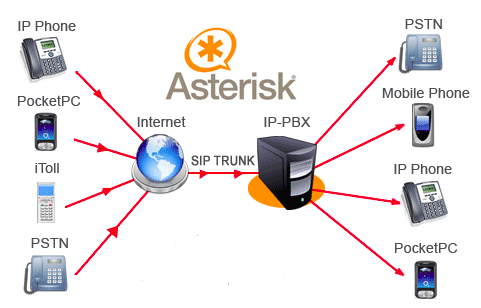
\includegraphics[width=0.5\textwidth]{img/asteriksvoip00.png}}
	\caption{Arquitectura de una red con \textit{Asterisk}}
	\label{fig:ant03}
\end{figure}
\textit{Asterisk} incluye muchas características que anteriormente sólo estaban disponibles en costosos sistemas propietarios PBX, como buzón de voz, conferencias, IVR, distribución automática de llamadas, y otras muchas. Los usuarios pueden crear nuevas funcionalidades escribiendo un dialplan en el lenguaje de script de \textit{Asterisk} o añadiendo módulos escritos en lenguaje C o en cualquier otro lenguaje de programación soportado en GNU/Linux.\\
Uno de los puntos fuertes del software \textit{Asterisk} es que permite la unificación de tecnologías: VoIP, GSM y PSTN.\\
\textit{Asterisk} se empieza a adoptar en algunos entornos corporativos como una gran solución de bajo coste junto con SER (Sip Express Router).


\subsection{\textbf{ FreePBX:}}  
\textit{FreePBX} es una GUI (interfaz gráfica de usuario) de código abierto basado en web que controla y dirige \textit{Asterisk}. \textit{FreePBX} está licenciado bajo la GNU General Public License y es un componente del FreePBX Distro (una distribución de GNU/Linux, basada en CentOS con el sistema PBX pre-instalado).
\begin{figure}[h]
	\centerline{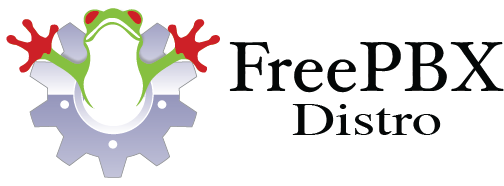
\includegraphics[width=0.25\textwidth]{img/freepbx01.png}}
	\caption{Logo de FreePBX Distro}
	\label{fig:ant04}
\end{figure}


\section{Desarrollo del concepto}\label{sec:ddc}
Para el desarrollo de nuestro proyecto, lo haremos de manera local por medio de una máquina virtual que hará de servidor

\section{Putamadre}
\subsection{Raspberry Pi 3}
Es el modelo más antiguo de la tercera generación de Raspberry Pi. Reemplazó el Raspberry Pi 2 Model B en febrero de 2016. Desarrollado en el Reino Unido por la fundación \textbf{Raspberry Pi}, con el objetivo de estimular la enseñanza de informática en las escuelas. \\
Salió a la luz en el año 2016, renueva procesador, una vez más de la compañía Broadcom, una vez más un Quad-Core, pero pasa de 900 MHz a 1.20 GHz. Mantiene la RAM de 1GB. Su novedad fue la inclusión de Wi-Fi y Bluetooth (4.1 Low Energy) sin necesidad de adaptadores.
\begin{figure}[h]
	%\centerline{\includegraphics[width=0.3\textwidth]{platform/rasp.jpg}}
	\caption{Raspberry Pi3 Modelo B.}
	\label{fig:ant01}
\end{figure}
Según Amazon, el precio está oscilando entre 50 y 70 dólares, dependiento del kit a comprar, donde incluyen módulos y memorias adicionales para su uso con la Raspberry.\\
Las características principales se las puede observar en el cuadro \ref{tab:rb01}.
\begin{table}[tbp]
\begin{center}
	\begin{tabular}{|p{2.5cm}|p{5.5cm}|}
	\hline 
	\textbf{Especificaciones} &\textbf{Raspberry Pi3 Modelo B} \\ \hline
	CPU  &1.2GHz 64-bit quad-core ARMv8 \\\hline
	Memoria (SDRAM) &1 GB compartidos con la GPU \\\hline
	Puertos USB &4 \\\hline
	Almacenamiento integrado &MicroSD \\\hline
	Conectividad de red &10/100 Ethernet RJ-45 vía hub USB, Wifi 802.11n, Bluetooth 4.1 \\\hline
	Fuente de alimentación &5 V vía micro USB o GPIO header \\\hline
	Sistemas Operativos Soportados &GNU/Linux: Debian (Raspbian), Fedora (Pidora), Arch Linux (Arch Linux ARM), Slackware Linux, SUSE Linux Enterprise Server for ARM. RISC OS.\\\hline
\end{tabular}\vspace{0.25cm}
\caption{Características Raspeberry Pi 3 Modelo B}
\label{tab:rb01}
\end{center}
\end{table}

	\subsection{Arduino Uno R3}
	El Arduino Uno R3 utiliza el microcontrolador ATmega328. En adición a todas las características de las tarjetas anteriores, el Arduino Uno utiliza el ATmega16U2 para el manejo de USB en lugar del 8U2 (o del FTDI encontrado en generaciones previas). Esto permite ratios de transferencia más rápidos y más memoria. No se necesitan drivers para Linux o Mac (el archivo inf para Windows es necesario y está incluido en el IDE de Arduino).\\
	\textbf{Arduino} es una compañía open source y open hardware, así como un proyecto y comunidad internacional que diseña y manufactura placas de desarrollo de hardware para construir dispositivos digitales y dispositivos interactivos que puedan sensar y controlar objetos del mundo real. \\
	El microcontrolador de la placa se programa usando el “Arduino Programming Language” (basado en Wiring) y el “Arduino Development Environment” (basado en Processing). Los proyectos de Arduino pueden ser autonomos o se pueden comunicar con software en ejecución en un ordenador (por ejemplo con Flash, Processing, MaxMSP, etc.).
	\begin{figure}[h]
	%\centerline{\includegraphics[width=0.25\textwidth]{platform/ardui}}
	\caption{Arduino Uno R3.}
	\label{fig:ardui}
	\end{figure}
	 El precio en Amazon oscila entre los 12 y 30 dólares, dependiendo del kit a comprar.\\
	Las características principales están presentes en el cuadro \ref{tab:ardui01}.
	\begin{table}[h]
\begin{center}
	\begin{tabular}{|p{2.5cm}|p{5.5cm}|}
	\hline 
	\textbf{Especificaciones} &\textbf{Arduino Uno R3} \\ \hline
	Microcontrolador  &ATmega328 \\\hline
	Voltaje de entrada &7 - 12 V \\\hline
	Entradas digitales &14 pines digitales de I/0 (6 salidas PWM) \\\hline
	Entradas analógicas & 6 entradas análogas \\\hline
	Memoria Flash &32k\\\hline
	Reloj &16MHz \\\hline
	Sistemas Operativos Soportados &N/A.\\\hline
\end{tabular}\vspace{0.25cm}
\caption{Características Arduino Uno R3}
\label{tab:ardui01}
\end{center}
\end{table}
	\subsection{Beaglebone black}
	Es una computadora barebone de desarrollo, la sucesora de la beaglebone lanzada en octubre de 2011. El precio está en 45 dólares y entre otras diferencias incrementa la RAM a 512 MB, el reloj de procesador a 1GHz, y añade HDMI y 2 GB de memoria flash eMMC. También se entrega con kernel Linux 3.8, permitiendo a la BeagleBone Black tener la ventaja del Gestor de Renderizado Directo (DRM).Demás especificaciones se observa en el cuadro \ref{tab:bb01}
		\begin{table}[h]
\begin{center}
	\begin{tabular}{|p{2.5cm}|p{5.5cm}|}
	\hline 
	\textbf{Especificaciones} &\textbf{BeagleBone Black} \\ \hline
	CPU  &Cortex-A8 + 2xPRU (200MHz) \\\hline
	Frecuencia SoC &1000MHz \\\hline
	DSP &DDR3 \\\hline
	Memoria & 512 \\\hline
	Memoria Flash &32k\\\hline
	Reloj &16MHz \\\hline
	Sistemas Operativos Soportados &Rowboat,Angstrom, Fedora, FreeBSD, MINIX 3, NetBSD, OpenBSD, openSUSE, QNX, RISC OS, Ubuntu, Void Linux, Windows Embedded.\\\hline
\end{tabular}\vspace{0.25cm}
\caption{Características BeagleBone Black}
\label{tab:bb01}
\end{center}
\end{table}
\begin{figure}[h]
	%\centerline{\includegraphics[width=0.2\textwidth]{platform/bb.jpg}}
	\caption{BeagleBone Black.}
	\label{fig:ant01}
\end{figure}
\subsection{pcDuino}
	\textbf{pcDuino} es una mini computadora o plataforma de computadora de una sola placa que funciona con PC como el sistema operativo, como Ubuntu y Android ICS. Da salida a la pantalla a HDMI. Además, tiene una interfaz de encabezados de hardware compatible con Arduino (TM). pcDuino puede usarse para enseñar Python, C y más cosas interesantes.\\
	\begin{figure}[h]
	%\centerline{\includegraphics[width=0.2\textwidth]{platform/pcd.png}}
	\caption{pcDuino1.}
	\label{fig:ant01}
\end{figure}
	\textit{pcDuino1} es una plataforma de mini PC rentable y de alto rendimiento que ejecuta PC como SO, como Ubuntu y Android ICS. Envía su pantalla a un televisor o monitor habilitado con HDMI a través de la interfaz HDMI incorporada. Está especialmente dirigido a las crecientes demandas de la comunidad de código abierto. La plataforma podría funcionar como un sistema operativo tipo PC completo con una cadena de herramientas fácil de usar y compatible con el popular ecosistema Arduino, como Arduino Shields (puede que necesite un puente protector) y proyectos de código abierto, etc. Las características principales se las observa en el cuadro \ref{tab:pcd01}.\\
			\begin{table}[h]
\begin{center}
	\begin{tabular}{|p{2.5cm}|p{5.5cm}|}
	\hline 
	\textbf{Especificaciones} &\textbf{pcDuino1} \\ \hline
	CPU  &1GHz ARM Cortex A8\\\hline
	DRAM &1 GB \\\hline
	Almacenamiento OnBoard &2GB Flash, microSD card slot hasta 32 GB \\\hline
	Interfaz de Red & 10/100Mbps RJ45 y USB Wifi extensión\\\hline
	Alimentación &5V, 2A\\\hline
	Sistemas Operativos Soportados &Linux3.0 + Ubuntu 12.04Android ICS 4.0\\\hline
\end{tabular}\vspace{0.25cm}
\caption{Características pcDuino1}
\label{tab:pcd01}
\end{center}
\end{table}
\section{Comparación de Plataformas}
Cada uno de estas mini computadoras tienen su correcto desarrollo dependiendo del aplicativo en el que le estén usando, es decir su uso dependerá de la función que lo pongas a realizar. La de menor escalabilidad podríamos mencionar a Arduino, ya que en primer lugar es un microcontrolador, y hay cosas en las que se queda corto, pero es ideal para llevar control de todo tipo de sensores y actadores y por su precio más todavía. Los restantes dependerá del sistema operativo a usarse, y los GPIOS que requeramos usar, si queremos un sistema operativo en tiempo real, la tasa de datos que queramos procesar, todas esas consideraciones hay que tener en cuenta al momento de escoger que plataforma utilizar.
\section{Conclusiones}
\begin{itemize}
	\item Las plataformas de prototipado permite elaborar a bajo costo operaciones de hardware por medio de periféricos de manera más sencilla.
	\item La utilización de las plataformas dependerá de la función que quiera realizar.
\end{itemize}
 
\begin{thebibliography}{00}
\bibitem{b1}  Liz upton, ``Introducing the New Out Of Box Software (NOOBS)'' , Raspberry Pi, 2013.
\bibitem{b2} Shead, Sam, ``Raspberry Pi delivery delays leave buyers hungry (and angry)", ZDNet, Octubre 2012.
\bibitem{b3} GSyC, ``Simple Network Managment Protocol,''  Universidad Rey Juan Carlos, 2013.
\bibitem{b4} LinkSprite, ``pcDuino1 Overview ,''  admin.
\bibitem{b5} ``OMAP3530 BeagleBoard" High perfomance and numerous expansion options; page 3, Dkc1.digikey.com , Mayo 2009.
\end{thebibliography}

\end{document}